%%%%%%%%%%%%%%%%%%%%%%%%%%%%%%%%%%%%%%%%%%%%%%%%%%%%%%%%%%%%%%%%%%%%%%%%%%%%%%%
%
% Background
% 
%%%%%%%%%%%%%%%%%%%%%%%%%%%%%%%%%%%%%%%%%%%%%%%%%%%%%%%%%%%%%%%%%%%%%%%%%%%%%%%

\chapter{Theoretical background}
\label{sec:background}

\section{Fluid-Structure Interaction}
Fluid-Structure Interaction (FSI) studies the interaction between a structure (solid) and a fluid flow (liquid or gas) around it. It is a multi-physics problem which has large interest in diversified fields such as mechanical engineering (e.g. airfoils), civil engineering (e.g. towers) or medicine technique (e.g. artificial heart valves). Based on the response of structure and fluid fields, it is classified as one-way or two-way fluid-structure interaction problem. If the structural displacement/deformation does not influence the flow fluid or vice versa, then the FSI system is termed to be one-way fluid-structure interaction system. Conversely if the fluid flow and the displacement or deformation of the structure have significant influence on each other then the FSI system is termed as two-way fluid-structure interaction problem. Figure \ref{fig:2.1} represents a typical domain of a fluid-structure interaction problem, $\Omega$ refers to the common domain, $ \Omega_{f} $ the fluid domain and $ \Omega_{s} $ the structure domain. Figure   \ref{fig:2.2a} and \ref{fig:2.2b} represents one-way and two-way FSI fluid-structure interaction problems respectively.\\

\begin{figure}[H]
	\centering
	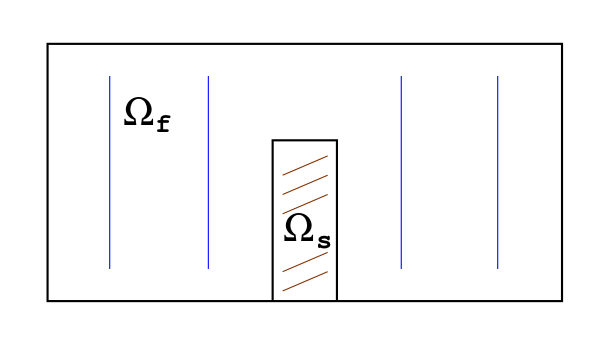
\includegraphics[height=3in]{fsi_domain}
	\caption{Representational figure of Fluid-Structure Interaction domain,taken from [cite 'Richter']}
	\label{fig:2.1}
\end{figure}

\begin{figure}[h]
  \centering
  \captionsetup{justification=centering}
  \begin{subfigure}[b]{0.8\linewidth}
    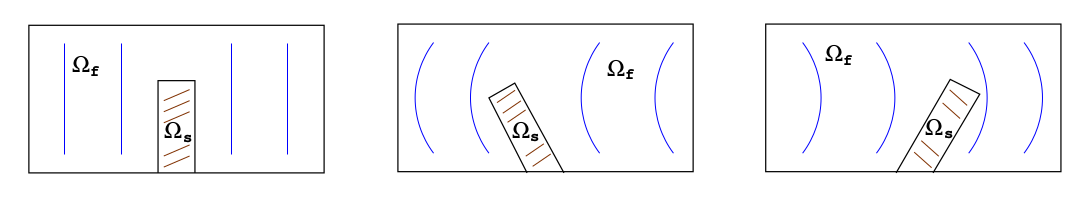
\includegraphics[width=\linewidth]{one-way-fsi}
    \caption{Structure domain influencing the fluid domain}
    \label{fig:2.2a}
  \end{subfigure}
  \begin{subfigure}[b]{0.8\linewidth}
    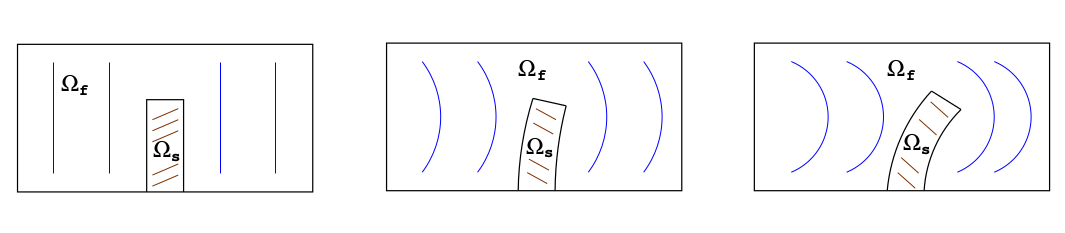
\includegraphics[width=\linewidth]{two-way-fsi}
    \caption{Both structure and fluid domains influencing each other}
    \label{fig:2.2b}
  \end{subfigure}
  \caption{Representational figure of one-way \ref{fig:2.2a}, and two-way \ref{fig:2.2b} fluid-structure interaction domains,taken from [cite 'Richter']}
  \label{fig:2.2}
\end{figure}

\subsection{Numerical simulation strategies of FSI problems}
Numerical simulation of FSI involves solving set of differential equations and corresponding boundary conditions for fluid and structural fields respectively. Suitable interface conditions needs to be defined so as the structural and fluid domains are well distinguished. There are different methodologies implemented to solve the FSI problem and are well documented in the literature. An overview of the numerical solution procedure for FSI problems are presented below.\\
The FSI problem is classified based on solution approaches and on the treatment of mesh handling techniques as represented below. A brief overview of these methods are presented subsequently.

\begin{itemize}
 \item{Classification based on numerical solution approaches}
 \begin{itemize}
 \item{Monolithic solver}
 \item{Partitioned solver}
 \begin{itemize}
 \item{Explicit coupling}
 \item{Implicit coupling}
 \end{itemize}
 \end{itemize}
 \item{Classification based on meshing strategies}
 \begin{itemize}
 \item{Conforming mesh}
 \item{Non-conforming mesh}
 \end{itemize}
\end{itemize} 

\subsubsection*{Classification based on numerical solution approaches}
This classification is based on how the fluid and structural fields are getting solved. In \textit{monolithic solvers} both the fluid and structural domains are expressed by single set of equations, whereas in \textit{partitioned solver approach} structural fields and fluid fields are solved separately and additionally requires coupling of the distinct solvers. A brief introduction to these methods are represented below.    

\subsubsection*{Monolithic solver approach}
The equations governing the fluid flow and the displacement/deformation of the structure are represented by single set of equations which are then solved simultaneously by an unified algorithm, within a single solver framework \citet{{Richter},{Becker_2014},{hubner2004monolithic},{michler2004monolithic}}. The central idea of monolithic solvers is to represent the interface by an homogeneous discretization, thus maintaining the conservation properties at the interface \citet{michler2004monolithic} \citet{van2003energy}. Although monolithic approach gives strong coupling between the fields, it is commonly considered to be impractical for real world applications. It also demands enormous computational power for solving such a large system of equations since it has to incorporate the behavior of both fluid flow and solid structure. Figure \ref{fig:2.3} represents a schematic of the monolithic and partitioned solver approaches in solving FSI problems.
    	  
\begin{figure}[h]
  \centering
  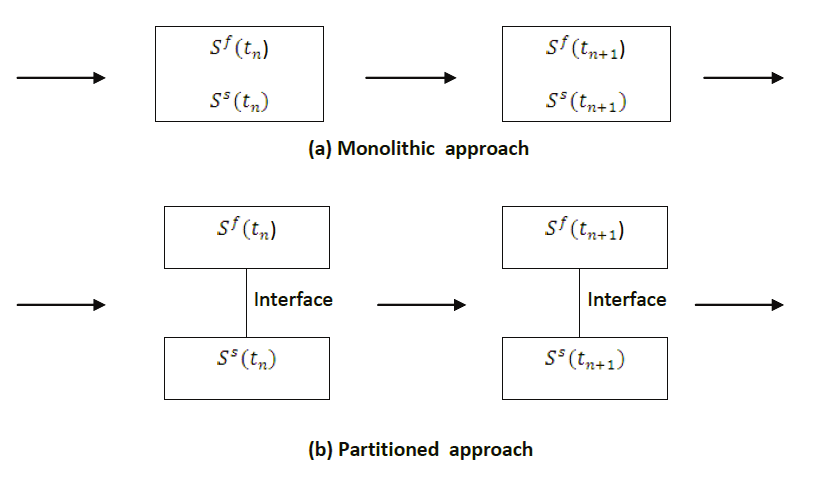
\includegraphics[width=1\linewidth]{monolithic}
  \caption{Schematic representation of Monolithic and Partitioned solution approaches. $ S^{f} $ represents the fluid solver and $ S^{s} $ represents the structural solver for two successive time steps current $ (t_{n}) $  and next $(t_{n+1})$. Figure taken from \citet{hou2012numerical}}
  \label{fig:2.3}
\end{figure}

\subsubsection*{Partitioned solver approach}
Another approach to fluid-structure interaction is to use two distinct solvers to model both fluid and solid domains. This technique allows the coupling of the fluid and solid solution by maintaining suitable coupling conditions. The interfacial conditions are used explicitly to communicate information between the fluid and structure solutions.\par

Some coupling algorithms were suggested by various studies (\citet{{piperno1995partitioned},{felippa2001partitioned},{farhat2000two}}) which allows for reuse of existing codes that have been developed for each field. This approach is very robust and can be used for wide variety of applications. The major disadvantage of this approach is that, the interface location that divides the fluid and the structure domains is not known apriori and usually changes in time. Thus, the partitioned approach requires tracking of the new interface location and its related quantities, which can be cumbersome and error-prone. The interface coupling conditions that are as stated below, have to be satisfied in order to have a stable solution.

\begin{itemize}
\item Kinematic coupling condition: The displacements, velocities and accelerations of the sub-zones have to be equal at the interface at any point in time.

$\psi^{CFD}_{\Gamma}(t) = \psi^{CSD}_{\Gamma}(t)$, $\dot{\psi}^{CFD}_{\Gamma}(t) = \dot{\psi}^{CSD}_{\Gamma}(t)$, $ \ddot{\psi}^{CFD}_{\Gamma}(t) = \ddot{\psi}^{CSD}_{\Gamma}(t) $

\item Dynamic coupling condition: Conservation of the dynamic equilibrium of all forces at the interface needs to be satisfied. (Action and reaction forces must cancel out each other)

$ f^{CFD}_{\Gamma}(t) = -f^{CSD}_{\Gamma}(t) $

\end{itemize}


Depending on the influence of the structure movement on the fluid field the FSI problems are further subdivided into two following categories:

\begin{itemize}
\item[Explicit/Weakly coupled:]	In an explicitly coupled algorithm, there is no 
\end{itemize}





